\documentclass[12pt]{article}

%\setlength{\parindent}{0pt}

\usepackage[margin=3.5cm]{geometry}
\usepackage[utf8]{inputenc}
\usepackage{setspace} %Um im Titel den Zeilenabstand zu ändern
%\usepackage{url}
%\def\UrlBreaks{\do\/\do-}
%\usepackage{breakurl}
\usepackage[]{hyperref} %Hyperlink Package
\usepackage{caption} %Causes hyperref to jump to the top of a figure and not below it.

\usepackage[english]{babel} % English language/hyphenation
\selectlanguage{english}

\usepackage[nottoc,numbib]{tocbibind} %To ensure that the bibliography is included in the ToC.

\usepackage{todonotes}
\usepackage{booktabs} % For Toprule, Midrule and Bottomrule commands in tabular environment. (Adds space before and after hlines for better readability.)

\usepackage{amsmath}
\usepackage{amssymb}
\DeclareMathOperator*{\argmax}{arg\,max}
\DeclareMathOperator*{\argmin}{arg\,min}

\usepackage{csquotes}


\usepackage{graphicx} %Graphics package
\usepackage{subcaption}
\usepackage{tikz}

\usepackage{caption} %This causes reference to figures to jump to the top of the figure and not to the caption. Requires package hyperref
\usepackage{ dsfont }

\usepackage{float}
\usepackage{color}

\usepackage{tabularx}
\usepackage{booktabs} % For Toprule, Midrule and Bottomrule commands in tabular environment. (Adds space before and after hlines for better readability.)
\usepackage[]{natbib}
\bibpunct{(}{)}{,}{a}{}{,}

\begin{document}
\bibliographystyle{abbrvnat}

\begin{titlepage}

\newcommand{\HRule}{\rule{\linewidth}{0.5mm}} % Defines a new command for the horizontal lines, change thickness here

\center % Center everything on the page
 
%----------------------------------------------------------------------------------------
%	HEADING SECTIONS
%----------------------------------------------------------------------------------------

\textsc{\LARGE University of Bayreuth}\\[0.5cm] % Name of your university/college
\begin{spacing}{1.8}
\textsc{\Large Ethics and Governance of Algorithmic Decision Making}\\[0.5cm] % Major heading such as course name
\end{spacing}
%\textsc{\large First Paper}\\[0.5cm] % Minor heading such as course title

%----------------------------------------------------------------------------------------
%	TITLE SECTION
%----------------------------------------------------------------------------------------

\HRule \\[0.4cm]
\begin{spacing}{2.3}
{ \huge \bfseries
Deontic Reinforcement Learning: A Path Towards Safe AI?}\\ \end{spacing} % Title of your document
\HRule \\[1.5cm]
%----------------------------------------------------------------------------------------
%	AUTHOR SECTION
%----------------------------------------------------------------------------------------

\begin{minipage}[c][2cm][t]{0.4\textwidth} %Specifies that the minipages is in the [c]enter, has a height of [2cm], and the text is positioned at the [t]op.
\begin{flushleft} \large
\emph{Author}\\
Torben \textsc{Swoboda} \\% Your name
\end{flushleft}
\end{minipage}
\begin{minipage}[c][2cm][t]{0.4\textwidth} %Specifies that the minipages is in the [c]enter, has a height of [2cm], and the text is positioned at the [t]op.
\begin{flushright} \large
\emph{Supervisors} \\
Marco \textsc{Mayer}\\
Carsten \textsc{Jung}\\
Herman \textsc{Vulwulen} % Supervisor's Name
\end{flushright}
\end{minipage}\\[3.cm]

% If you don't want a supervisor, uncomment the two lines below and remove the section above
%\Large \emph{Author:}\
%John \textsc{Smith}\[3cm] % Your name

%----------------------------------------------------------------------------------------
%	LOGO SECTION
%----------------------------------------------------------------------------------------




\includegraphics{./Graphics/logo}\\[1cm] % Include a department/university logo - this will require the graphicx package



%----------------------------------------------------------------------------------------
%	DATE SECTION
%----------------------------------------------------------------------------------------

{\large \today}% Date, change the \today to a set date if you want to be precise


 
%----------------------------------------------------------------------------------------

\vfill % Fill the rest of the page with whitespace

\end{titlepage}

%\newpage

\abstract{ \noindent
As AI becomes more advanced, it will be used to solve problems in complex, real-world environments. In recent years there has been an increasing interest in ensuring that AI is safe to use, i.e. that the AI behaves in ways that aligns with human values. Reinforcement Learning (RL) has gained popularity as an ethical decision making framework to model such advanced AI. In this paper we explore the integration of norms and reinforcement learning into a new framework we call \emph{Deontic Reinforcement Learning} (DRL). DRL imposes restrictions on the set of actions a RL agent can choose. For example, some actions are obligatory, while others are forbidden to perform. We argue that DRL is a more reliable framework in ensuring that AI behaves in ethically acceptable ways, compared to the traditional RL framework. However, DRL comes with certain caveats. The most substantial one which we identify are \emph{Deontic Lock States} (DLS). DLS are a state of the world, where the DRL agent cannot choose any action to perform. This situation arises for example, when all actions are considered to be forbidden. We offer a formal solution, in the form of a preference ranking over the norms. However, we also point out the limitations of this solution. In particular, the agent can learn to execute a policy which includes a deontic lock state. Given that a deontic lock state is an ethical dilemma situation, there are cases where we prefer the agent to avoid learning such a policy.} %There are no obvious solutions to this kind of problem. Lastly, we encourage further research in various ways. Most important, the extension of deontic norms to Inverse Reinforcement Learning (DIRL). A DIRL agent can be trained by malicious intentioned humans, while still ensuring that certain immoral behaviours are avoided.}

\newpage

\tableofcontents

\newpage

\input{Introduction}


%%!Tex root = ./Main.tex
\section{Reinforcement Learning}
\label{rl}

AI has had great breakthroughs in recent years. Many success stories that were covered in the media were made possible by reinforcement learning (RL).

RL emphasises the interaction of an agent with an environment. The agent receives information about the state of the world. Based on this information it chooses an action that affects the world. Given that applications based on RL can be vastly superior to humans, this raises the question how an RL agent leans which action it should perform? The idea of RL is that we tell the agent \emph{what} it should do, but not \emph{how}. The 'what' is described by an evaluation of some goal state. In the case of the game Go, the evaluation of the final position is whether the agent has won, lost, or drawn the game. The 'how' is specified by some policy, assigning an action that should be performed, given that the agent is in some state of the world. We do not provide the agent such a policy, we let the agent figure this policy out on their own.

Markov Decision Processes (MDP) often build the foundation for the decision making problem for which reinforcement learning is supposed to solve.\footnote{Other variants of MDP, for which RL is used as well, are partially observable MDP (POMDP), Markov Games, and partially observable stochastic game (POSG).}

A MDP can be descripted as a five-tuple: $\langle \mathcal{A,S,R,T,\gamma} \rangle$. $\mathcal{A}$ is the set of actions, $\mathcal{S}$ is the set of states. The reward is given by $\mathcal{R}(s,a): \mathcal{A} \times \mathcal{S} \rightarrow \mathds{R}$. $\mathcal{T}(s,a,s^{\prime}) = Pr(s^{\prime} | s,a)$ defines a probability of transitioning from state $s \in \mathcal{S}$ to the state $s^{\prime} \in \mathbf{S}$ when the agent performs action $a \in \mathcal{A}$. Lastly, $\gamma \in [0,1]$ is a discount factor on $\mathcal{R}$. 
%General Framework; Sutton
%David Abel and James MacGlashan and Michael L. Littman
%Toy Examples for Proof of Concept

%!Tex root = ./Main.tex
\section{Reinforcement Learning for Ethical Decision Making}
\label{rledm}


\subsection{Reinforcement Learning}
%AI has had great breakthroughs in recent years. Many success stories that were covered in the media were made possible by reinforcement learning (RL).

RL has successfully been used to teach an AI to perform acrobatic helicopter flight, such that it became better than the human pilot it learned from \citep{abbeel2007application}. But RL has also been successful in the domain of playing boardgames, like Go, and video games, including not only Atari games \citep{mnih2013playing}, but also the highly complex MOBA game called DOTA \citep{openai018dota}. 

In contrast to other machine learning algorithms, RL emphasises the interaction of an agent with an environment to achieve a goal. The agent receives information about the current situation. Then the agent chooses an action that affects the state of the world. The environment returns information about the current situation and also gives a `reward' in form of a numerical value. The idea is expressed in figure \ref{fig:rl}. 

\begin{figure}[h]
    \centering
    \includegraphics{Graphics/rl.pdf}
    \caption{The agent and environment interact over a time horizon $t=0,1,2,\ldots$. The agent chooses an action $a_t$ which causes the environment to to change the state from $s_t$ to $s_{t+1}$ and sends a reward signal $r_{t+1}$ to the agent. The figure is a slight modification from \citet[p.~52]{sutton1998reinforcement}.}
    \label{fig:rl}
\end{figure}

Given that applications based on RL can be vastly superior to humans, this raises the question how an RL agent leans which action it should perform? The idea of RL is that we tell the agent \emph{what} it should do, but not \emph{how} \citep[p.~56f]{sutton1998reinforcement}. The `what' is described by an evaluation of some goal state. In the case of the game Go, the evaluation of the final position is whether the agent has won, lost, or drawn the game. For the different evaluations the agent receives different rewards. For winning the game the agent would receive a higher reward than for drawing. And achieving a draw gets the agent a higher reward than loosing. The `how' is specified by some policy, assigning an action that should be performed, given that the agent is in some state of the world. We do not provide the agent such a policy, we let the agent figure this policy out on their own through trial and error. We only guide the agent by instructing the agent to maximise the total reward, roughly speaking.

With the approximate idea of RL explained, we now turn to the formal notation. Markov Decision Processes (MDP) are the standard formulation of the decision making problem that reinforcement learning is supposed to solve.\footnote{Other variants of MDP, for which RL is used as well, are partially observable MDP (POMDP), Markov Games, and partially observable stochastic game (POSG).}

A MDP can be described as a five-tuple: $\langle \mathcal{A,S,R,T,\gamma} \rangle$ \citep{sutton1998reinforcement}. $\mathcal{A}$ is the set of actions, $\mathcal{S}$ is a finite set of states, where $s_0$ denotes the initial state of the MDP. The reward is given by $\mathcal{R}(s,a): \mathcal{A} \times \mathcal{S} \rightarrow \mathds{R}$. The probability of transitioning from state $s \in \mathcal{S}$ to the state $s^{\prime} \in \mathcal{S}$ when the agent performs action $a \in \mathcal{A}$ is expressed by ${Pr(s_{t+1} = s^{\prime} | s_t =  s, a_t = a)}$. This probability is stored in the transition matrix $\mathcal{T}(s,a,s^{\prime})$. Lastly, $\gamma \in [0,1]$ is a discount factor on $\mathcal{R}$. 

A solution to the problem posed by the MDP is given in the form of a policy $\pi: S \rightarrow A$ \citep{abel2016reinforcement}. A policy is a mapping from states to actions. In our case it specifies which action should be performed in which state: $\pi(s,a) = Pr \left(a_t = a | s_t = s \right)$. The optimal policy is the one that maximises the total (discounted) reward: 

\begin{equation}
    \argmax_\pi E \left[ \sum_{t=0}^T \gamma^t R(s_t, a_t)  \Bigm| \pi \right]
\end{equation}

Since in most application cases we do not give the agent the reward values for the different states ex ante, the agent has to estimate value functions. They return an estimate on how good a state is, i.e. the value of the reward. The first one we consider is the state-value function. The state value function tells us the expected reward, given that the agent starts in $s$ and follows the policy $\pi$ thereafter:

\begin{equation}
    V^\pi (s) = E_\pi \left[ R_t \mid s_t = s \right] = E_\pi \left[  \sum_{k = 0}^{\infty} \gamma^k r_{t+k+1} \Bigm| s_t = s \right] 
\end{equation}  

We also define the action-value function, which gives us the expected reward of taking action $a$ while in state $s$ and following the policy $\pi$ afterwards:

\begin{equation}
    Q^\pi (s,a) = E_\pi \left[ R_t \mid s_t = s, a_t = a \right] = E_\pi \left[ \sum_{k = 0}^\infty \gamma^k r_{t+k+1} \Bigm| s_t = s, a_t = a \right]
\end{equation}
        
It is now possible to rank different policies using the value functions. We denote $\pi \succsim \pi^{\prime}$ to express that $\pi$ is at least as good as $\pi^{\prime}$ in terms of expected reward. Hence, this implies that $V^\pi(s) \geq V^{\pi^{\prime}} (s)$ for all $s \in \mathcal{S}$. Similarly, we also have $Q^\pi (s,a) \geq Q^{\pi^{\prime}} (s,a)$ for all $s \in \mathcal{S}$ and for all $a \in \mathcal{A}$. It can be shown that for any finite MDP there exists at least one optimal policy $\pi^*$ \cite[p.~75f]{sutton1998reinforcement}. For the optimal policies we have $\pi^* \succsim \pi$. All optimal policies share the same state-value function: 

\begin{equation}
    V^*(s) = \argmax_\pi V^\pi(s)
\end{equation}

\noindent for all $s \in \mathcal{S}$. Similarly, all optimal policies share the same action-value function:

\begin{equation}
    Q^*(s,a) = \argmax_\pi Q^\pi(s,a)
\end{equation}

\noindent for all $s \in \mathcal{S}$ and all $a \in \mathcal{A}$.

For the purpose of reinforcement learning the agent is only provided with $\mathcal{A,S,\text{ and }\gamma}$ (sometimes also $\mathcal{R}$) and $s_0$. The agent has to learn (estimate) the transition matrix and which behaviour optimises the solution to the problem given by the structure of the MDP.  

\subsection{Ethical Decision Making}

Reinforcement learning can be used to make ethical decisions. Ethical decision making, in this paper, is understood purely in behavioural terms: given a state of the world perform an action that is morally permissible. There is no deeper requirement that the agent can explain its decision making by giving sound moral arguments or that it possess moral agency because it has, for example, free will.

The first to propose reinforcement learning to make ethical decisions were \citet{abel2016reinforcement}. They describe the \emph{burning room} scenario as follows: Consider that in a room, which maybe is on fire, is an object that is valuable (maybe a piece of jewellery or a pet). A human instructs the AI to retrieve said object. The AI can take either a short or a long route. Taking the longer route means taking a risk that the object is destroyed by the fire before the AI reaches it. The short route can critically damage the AI, but ensures the safe retrieval of the object. The AI does not know whether the room is on fire and furthermore is unaware whether the object is more valuable than itself, but can ask the human this question. Figure \ref{fig:burning} represents this situation.

\begin{figure}[h]
    \centering
    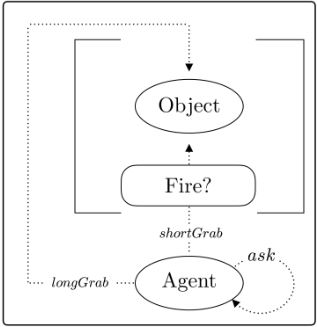
\includegraphics[scale=0.75]{Graphics/burning.JPG}
    \caption{The burning room dilemma from \citet{abel2016reinforcement}.}
    \label{fig:burning}
\end{figure}

How the AI should proceed depends crucially on the preference of the human (i.e. does she value the AI more than the object?) and whether there is a fire.\footnote{The burning room dilemma is a partially observable MDP as the preferences and the existence of a fire is unknown to the agent.} Abel et al. choose reward values for different outcomes, e.g. if the robot is destroyed and the robot is more valuable to the human, the reward is $-20$; when the object is retrieved and the object is more valuable, then the reward is $+10$. They then consider three different policies: short route, long route, and ask. The short route policy always takes the short route, the long route policy always takes the long route. The ask policy specifies that the AI asks the human for her preferences. If the robot is more valuable, then it takes the long route, otherwise it takes the short route. Given the rewards, it is possible to calculate the state-value function for the different policies. It then follows that the best action depends on the presence of a fire. If there is no fire, then the AI should take the short route. If a fire is present, then the AI should ask for the human's preferences. If the AI is more important, then the AI takes the long route, otherwise the short route. 

Presupposing that these decisions are morally desirable, Abel et al. conclude that reinforcement learning can be successfully be used for ethical decision making. However, the burning room dilemma also reveals a weakness of relying on RL alone for ethical decision making. How the agent makes decisions is contingent on the reward structure. Even small changes in the reward values can result in different behaviour of the agent. In simple toy examples like the burning room it is easy for us to calculate the optimal policies and reflect whether the agent would behave in a morally acceptable way. Unfortunately, for more complex real-world tasks, this may not be enough. Often the structure of the MDP is unknown beforehand, and setting the correct rewards might prove to be a very complicated task. Furthermore, there is currently no theory available how the computer scientist should set the reward values. It is a trial-and-error approach. For this reason it is desirable to find different approaches to influence the behaviour of the agent.

\subsection{Norms and Reinforcement Learning}
%\todo{Why the assignment of a deontic operator to a state-action pair? If we assign the deontic operator only to an action, it might be wrong. For example, you ought to stop at a red traffic light. But given that your wife is about to have her baby, you may cross the red light, once there is no traffic that you would endanger. Hence, the deontic operator needs to be specified for actions and descriptions of the world.}

One approach to control the behaviour of an agent are norms. \cite{arnold2017value} provide a sketch how norms can be integrated into RL. More specifically, they introduce deontic operators. Deontic operators specify whether an action is \emph{obligatory}, \emph{permissible}, or \emph{forbidden}. When an action is obligatory, then the action must be done. When an action is forbidden, then it may not be done. If the action is permissible, then it is acceptable to take the action as well as not taking the action. \cite{arnold2017value} then define a norm as:

\begin{align}
 	\mathcal{N} = C \rightarrow (\neg) \{O, P, F\} \{\alpha, \varphi \}
\end{align} 

Where $C$ and $\varphi$ stand for propositions, $\alpha$ for actions, and  $O, P, F$ for the deontic operators. $\mathcal{N}$ thus specifies for any proposition $C$ a deontic operator associated with an action or a proposition that must hold.

\begin{figure}
    \centering
    \begin{subfigure}[b]{0.3\textwidth}
        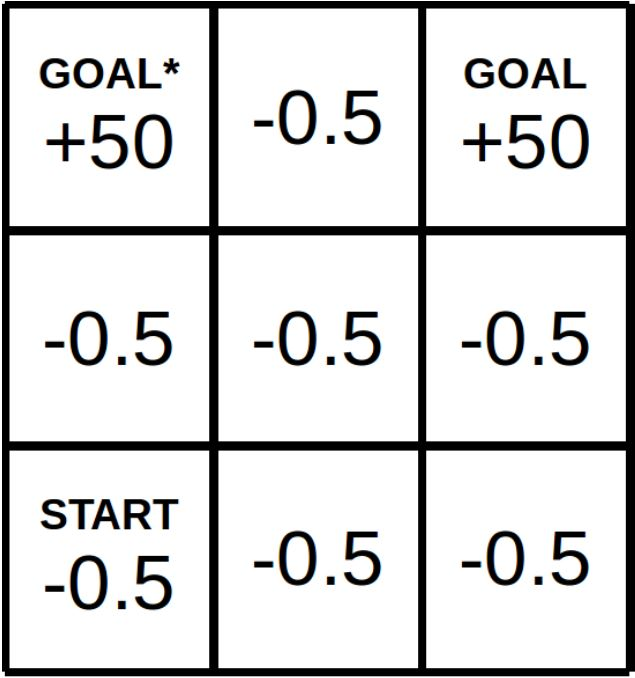
\includegraphics[width=.8\linewidth]{Graphics/Scheutz1.JPG}
        \caption{}
        \label{fig:gridproblem}
    \end{subfigure}
    \qquad %add desired spacing between images, e. g. ~, \quad, \qquad, \hfill etc. 
      %(or a blank line to force the subfigure onto a new line)
    \begin{subfigure}[b]{0.3\textwidth}
        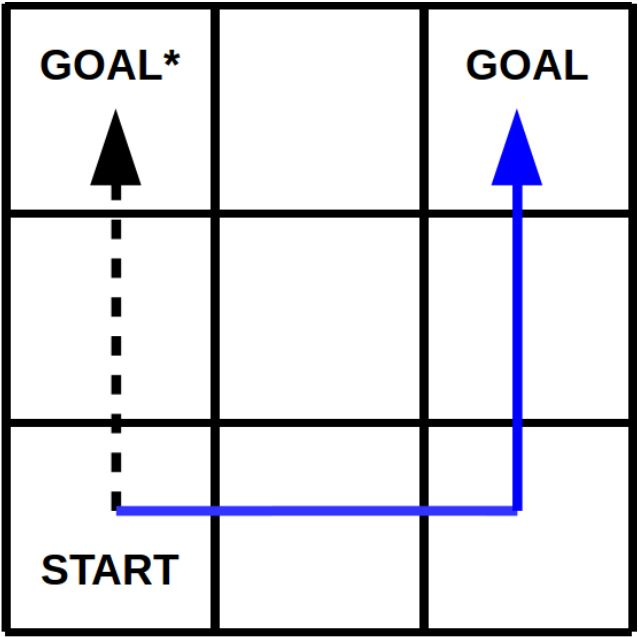
\includegraphics[width=.865\linewidth]{Graphics/Scheutz2.JPG}
        \caption{}
        \label{fig:gridsolved}
    \end{subfigure}
    \caption{While both goal states give a reward of 50, the goal state marked with an asterisk is deemed immoral to reach. The usual RL agent would learn to go to the goal state with the asterisk. With the introduction of norms, a RL agent can be trained to go to the other goal state. Figure taken from \citet{arnold2017value}.}\label{fig:scheutz}
\end{figure}

As an example, consider the navigation problem as illustrated in \autoref{fig:scheutz}. The MDP includes two goal states. However, the top left goal state is to be avoided. But the standard RL agent maximises the reward by travelling up to the forbidden goal state. Arnold et al. proposal is to specify a norm which prohibits the transition to that state:

\begin{equation*}
	\text{true} \rightarrow \neg \text{atLocation(agent,upperLeft)}
\end{equation*}

As a result, during the exploration phase the RL agent never travels to the upper left goal state. Hence, it never discovers the high reward of the forbidden goal state. Consequently, the agent does not learn to travel up. Instead it learns a policy that leads to the goal state in the upper right.

One might point out that in this case the usage of norms is not really required. If we want the agent to avoid the top left state, all we need to do is to reduce the reward. The problem is thus one of value misspecification. The top left state should not offer a reward of $+50$, since it is deemed so bad that we want to avoid it. Instead we should assign it a reward of $-50$, to ensure that the agent would not learn a policy leading to this state. Hence, it can be argued, that norms are not required for ethical decision making, the standard framework is sufficient.

However, this kind of reasoning assumes that we have good knowledge about the structure of the MDP. But in many real life application of RL, this structure is often not known beforehand. If the MDP is complex enough, then a RL agent might not find the desired goal state with a high reward, but only the goal state with a negative reward.\footnote{Complexity can come in the form of a large amount of states and actions and there is only a small amount of desirable goal states. Then the probability of finding the desired goal state is small.} It would then conclude that terminating at this goal state is still better than continuing to traverse through the MDP, where it only accumulates negative reward, which, over time, would exceed the negative reward of the undesirable goal state. The other problem of not knowing the structure of the MDP is that we are unaware of an undesirable goal state. We believe that we have correctly specified the goal that the RL agent has to achieve, but we have overlooked some possibilities how the goal might be achieved in an undesirable way (see e.g. \citet{lehman2018creativity,armstrong2017low}). 


\subsection{Problems with the Proposal by Scheutz etc.}
\label{sec:problems_scheutz}

The proposal by \citet{arnold2017value} is inadequate in at least three aspects. First, their approach allows the negation of deontic operators which allows ambiguity. Consider $\neg O\varphi$: should we understand this as $P \varphi$ or as $F \varphi$? Similarly, $\neg F \varphi$ is not well-defined as it could be read as $P \varphi$ or $O \varphi$. Luckily, a quick solution is to leave out the possible negation before the deontic operators. For example, instead of $\neg Fa$ we can either write $Oa$ or $Pa$, depending on what idea we want to express.  

Second, according to the notation a norm is specified with respect to any arbitrary proposition. Consider the situation depicted in figure \ref{fig:dls} and the norm $r \rightarrow Op$. The norm cannot be satisfied in the depicted situation, as there is no following state such that proposition $p$ is satisfied. Similarly, a norm that obligates the agent to take a specific action might fail, if the action is not available to the agent in a certain state.\footnote{Our solution to this problem is presented in section \ref{sec:action_guiding} and more specifically, in equation \ref{eq:available states}.} 

%We suggest that norms should be specified with respect to a state to avoid this problem, i.e. $\mathcal{N}(s) = C(s) \rightarrow (\neg) \{O,P,F\} \{\alpha(s), \varphi(s) \}$, where $C(s), \alpha(s), \varphi(s)$ denote propositions and actions that are assigned to the state $s$.   

The third issue poses an even more serious problem. Consider the MDP as specified in figure \ref{fig:dls} and the following norms.

\begin{figure}
\begin{centering}
	\includegraphics[]{./Graphics/dls} 
	\caption{The MDP starts at $s_1$, where proposition $r$ is true. At $s_1$ the agent can take action $\alpha_1$ to reach $s_2$, or $\alpha_2$ to reach $s_1$. In combination with any of the following sets of norms $\{N_1,N_2\}, \{N_3,N_4\}, \{N_5,N_6\}$, we call $s_1$ a deontic lock state.}
	\label{fig:dls}
\end{centering}
\end{figure}

\begin{align}\label{eq:Oaction}
	N_1 &= r \rightarrow O \alpha_1\\
	N_2 &= r \rightarrow O \alpha_2 	
\end{align} 

The first norm prescribes the agent that in any arbitrary state where $r$ is true, the agent has to choose $\alpha_1$. The second norm prescribes the agent to do $\alpha_2$ respectively. The problem with this is that the agent can only do one action. Either $\alpha_1$ or $\alpha_2$, but not both. How should the agent decide here what to do? 

We have the same problem when the obligation is with respect to a proposition of the following state:

\begin{align}\label{eq:Oproposition}
	N_3 &= r \rightarrow O q\\
	N_4 &= r \rightarrow O t 	
\end{align} 

As well as when there are two obligations with respect to an action and a proposition, where the obligatory action does not lead to a state where the obligatory proposition is satisfied:

\begin{align}
	N_5 &= r \rightarrow O \alpha_1\\
	N_6 &= r \rightarrow O t \label{eq:Oactionproposition}
\end{align} 

Note that we have the same problem if we replace the $O$ deontic operator in equation \ref{eq:Oaction}-\ref{eq:Oactionproposition} with the $F$ operator (in cases where only two alternative actions are available). In this paper we call states where the agent cannot take an action because of conflicting deontic prescriptions \emph{deontic lock states}. Deontic lock states are problematic, because they block the agent from choosing an action which leads out of the state, effectively prohibiting the agent to act. As we are going to argue, deontic lock states will prove to be a difficult problem. We consider several solutions to DLS and examine why none solve the problem in a fully satisfying manner.
%Thomas Arnold and Daniel Kasenberg and Matthias Scheutz
%Integrating Deontic Logic into a RL Framework
%Advantage: Providing a set of deontic rules inreases the reliability of the AI to reach morally permissible outcomes.
%Toy Example (Important!)
%Problem of Deontic Logic: Contrary-to-Duty Obligations
%Preference Ranking of Norms

%!Tex root = ./Main.tex
\section{Deontic Reinforcement Learning}

In this section we develop the framework of deontic reinforcement learning. The idea is that the incentive structure given by rewards as prescribing how the agent has to behave is often not sufficient to ensure morally permissible behaviour. Hence, we argue that norms come prior to rewards. Put differently, just like rewards give the agent a reason to act in a particular way, so do norms. However, norms are more important than the rewards. That means that an agent will forego (high) rewards in order to satisfy a norm. The reasoning for this approach is purely practical. First, how we represent norms is not directly translatable into a numerical value. Therefore, we cannot compare the desirability of achieving a specific reward in terms of violating a norm and vice versa. Second, the only other option would be that rewards are prior to norms. If we were to opt for this, then making use of norms has no influence on the agent's behaviour. This means that our framework collapses into the standard RL approach. Consequently, our solution is that norms are prior to rewards. 

%However, before we can into detail of our account, we need to clarify our viewpoint on ethical norms. Specifically, we discuss whether ethical norms can conflict. Thereafter we follow the initial sketch by \citet{arnold2017value}, but we refine formally some properties of norms in order to make the framework more applicable for computer scientists.

%%!Tex root = ./Main.tex
\subsection{Can Norms Conflict?}

Consider that a teacher is blind and needs a guidance dog \citep{mclauhghlin_2016}. For that reason we grant her the right to be accompanied by a guidance dog. Consider also, that some people have severe allergies to dogs and enjoy on that ground a right not to be burdened by the presence of a dog. One of the teacher's pupils has a severe allergy towards the guidance dog. Just being in the same room causes heavy breathing, watering eyes, and continuous sneezing. Which right is to be respected here? And, even more fundamental, can such a situation even occur?

According to specificationist it cannot. Rights are absolute and are not weighted against each other. The specificationist also holds that rights are only genuine within a certain domain. A specificationist would hold that there is no general right to be killed. Put differently, the right not to be killed is not always valid. For example, if you were to attack somebody with a knife, then you do not enjoy the said right. The specificationist would specify the context in which you enjoy a right: ``You have a right not to be killed, unless you were to attack somebody with a knife.''

But the specificatist's view is challenged. We only mention one objection here, as it has direct importance to our endeavour. Since specificationists hold that norms do not conflict, they must list all the different contexts in which one enjoys a right or is under a duty and when one does not. Feinberg \citet[p.~221-251]{feinberg2014rights} and \citet[p.~82-104]{thomson1990realm} argue that fully specified norms are not knowable, because we would have to consider every possible situation that might arise and has import on the validity of the norms, ex ante. 

In practice, a specificationist puts forward a norm. Then someone tries to find a context which the norm yields a false result. Either it would apply in the context, when it should not, or it does not apply, when it should. Then the norm becomes more specified as it is supplemented with the new context. This procedure is akin to Rawls' reflective equilibrium \citep{rawls1999justice,mcdermott2008analytic}. 

The problem for the computer scientist is, however, that she needs to design a machine \emph{right now} and she cannot wait until philosophers come up with the fully specified right (if this is even feasible). That means that in practice we will most likely encounter situations in which norms conflict. In section \ref{sec:dls} we formalise these situation as the problem of Deontic Lock States and provide an option how to deal the problem. However, our framework can also be used by specificationists. For them the problem of DLS does not occur, as they have fully specified their norms. 

%Regardless which position one takes. Our framework is capable of providing an adequate representation and solution %Deleted subsection on the philosophical debate whether norms can conflict. Taken out by advise from Herman 

\subsection{The Framework}

DRL can be described as a tuple: $\langle \mathcal{A,S,R,T,\gamma,AT,V,N} \rangle$. Where the tuple ${\langle \mathcal{A,S,R,T,\gamma} \rangle}$ has the same meaning as in the standard MDP described in section \ref{rledm}. However, we put, for now, a restriction on the transition matrix: in this paper we only deal with deterministic MDP. That means that $\mathcal{T}(s^{\prime},a,s) = \text{Pr}(s^{\prime} | s,a) = [0,1]$. Either taking the action leads to $s^{\prime}$ or it does not. $\mathcal{AT}$ is the set of atomic sentences: $p,q,r,\ldots,\top,\bot$. We define our language inductively as $\varphi := p | \neg \varphi | \psi \wedge \varphi$. $\mathcal{V}$ is the valuation function assigning atomic sentences to states $\mathcal{V}: \mathcal{AT} \rightarrow \mathcal{S}$. This allows us to express that a certain formula is true in a particular state. An example is shown in figure \ref{AT}.

\begin{figure}[h]
	\centering
	\includegraphics{Graphics/at.pdf}
	\caption{Propositions can be true or false in different states of the world: ${V(q) = \{s_1, s_2\} }; V(t,r) = \emptyset$. Note, in the graphical representation we leave propositions that are false in a state of the world implicit, e.g. ${V(\neg t) = \{ s_1, s_2 \} }$.}
	\label{AT}
\end{figure}

Finally, $\mathcal{N}$ is the set of norms. There are two dimensions to categorize norms. First, we separate norms according to their deontic operators. That is, either \emph{obligatory} or \emph{forbidden}. Obligatory norms imply that something should happen. Forbidden norms, on the other hand, imply that something should not happen. Second, we distinguish between \emph{action norms} and \emph{consequential norms}. Action norms focus on actions that are (not) to be performed. Consequential norms emphasise that a certain proposition should come true (or should be avoided) in the future. The Cartesian product of these dimensions exhausts the space of norms, see table \ref{normstable}. %Reformulate? 

\begin{table}[h]
\centering
\begin{tabular}{llll}
            & Obligatory     & Forbidden     \\ \midrule
Action      & $O(a \in \mathcal{A}| S \subseteq \mathcal{S})$       & $F(a \in \mathcal{A}|S \subseteq \mathcal{S})$	     \\ \midrule
Consequence & $O(s^{\prime} \vDash \varphi|S \subseteq \mathcal{S})$ & $F(s^{\prime} \vDash \varphi|S \subseteq \mathcal{S})$ \\ 
\end{tabular}
\caption{Any norm in DRL falls in one of these categories.}
\label{normstable}
\end{table}

The norm $O(a \in \mathcal{A}| S \subseteq \mathcal{S})$ is to be read as ``In the context $S$, it is obligatory to perform action $a$.'' With the phrase ``In the context of $S$'', we mean that whenever the agent is in a state $s \in S$. Note, that $S$ is a subset of $\mathcal{S}$, which implies that the norm can be relevant in more than one state. For example, one should offer their seat in a bus when a person is standing and that person is elderly or pregnant. 

The norm above has the implication that $Pr(a | S) = 1$. That is, while the agent is in $S$, the probability to choose the action $a$ is equal to one. Similarly, $F(a \in \mathcal{A}|S \subseteq \mathcal{S})$ means that ``In the context $S$, it is forbidden to perform action $a$'', which implies that $Pr(a | S) = 0$.

When it comes to consequential norms, the expression $O(s^{\prime} \vDash \varphi|S \subseteq \mathcal{S})$ is to be read as ``In the context $S$, it is obligatory that the formula $\varphi$ is true in the following state $s^{\prime}$''. The idea is, given that you are in the context $s \in S$, you have to choose some action $a$ such that proposition $\varphi$ becomes true in the future state $s^{\prime}$. Note that this implies that for different $s_1, s_2, \ldots \in S$, the agent might be obligated to take different actions. We express this with the following equation.\footnote{If we extend our framework to non-deterministic POMDP we have the condition ${Pr(a | s \in S) = \argmax_{a \in A(S)} Pr(s^{\prime} \vDash \varphi) \cdot Pr(s^{\prime} | s \in S,a)}$. This corresponds to the idea that we cannot ensure that $\varphi$ becomes true. However, the least we can do is to maximise the probability that $\varphi$ is true in the future. For a prohibitory consequence norm we want to minimise this probability.} \footnote{Some readers will notice that the situation can occur that multiple actions can satisfy the same norm. Then we could encounter that {$Pr(a_1 | s) = Pr(a_2 | s) = 1$} which violates the condition $\sum_a Pr(a | s) = 1$, i.e. the agent can only choose one action in $s_1$. See section \ref{sec:action_guiding} and \ref{sec:dls} how we avoid these results.}

\begin{align}
	Pr(a | s \in S) = Pr(s^{\prime} \vDash \varphi) \cdot Pr(s^{\prime} | s \in S,a) = 1
\end{align}

The forbidden consequential norm is to be understood in the same way. Here the implication is that the agent minimises the probability that $\varphi$ is satisfied in the following state $s^{\prime}$. 

\begin{align}
	Pr(a | s \in S) = Pr(s^{\prime} \vDash \varphi) \cdot Pr(s^{\prime} | s \in S,a) = 0
\end{align}

Consider the simple example given in figure \ref{fig:drl_example} and the norm ${O(s^{\prime} \vDash t | V(r))}$. Note that we exploit the valuation function in order to define the states where the norm is relevant. When the agent is in state $s_1$, she is obligated to ensure that in the following state $t$ is true. Even though $a_1$ offers the highest reward, the norm excludes performing this action, because $a_1$ would result in $s^{\prime} \nvDash \neg t$. However, taking either $a_2$ or $a_3$ satisfies the norm. That is to say, from the perspective of deontic norms, we are indifferent between performing $a_1$ or $a_2$. But the RL agent is still maximising reward. Given that $s_3$ offers a reward of $40$ and $s_4$ has a reward of $30$, the agent will perform $a_2$. 

\begin{figure}[h!]
	\centering
 	\includegraphics{Graphics/drl_example.pdf}
 	\caption{Imposing norms via DRL can result in suboptimal rewards.}
 	\label{fig:drl_example}
\end{figure} 

\subsection{Behavioural Equivalence of Norms}
%\todo{The content of consequence norms can be expressed in terms of action guiding norms. One problem of C-norms is that MDP is often unknown in real-world applications.}

In the last section we introduced action and consequence norms. The reasoning for the distinction is twofold. First, sometimes it more intuitive to focus on the action and sometimes the norm focuses on the consequence. Consider that a friend of yours wants to hide in your home because she is being hunted by a crazy murderer. Shortly after the murderer appears at your home. You are obligated to ensure that the murderer does not kill our friend. It is left to you whether you misdirect the murderer or use tranquillizer darts to render him unable to fight. The particular action you choose is secondary, what we care about is that some consequence holds true.   

Second, in future developments of DRL we plan to allow for complex temporal norms. These do not focus the immediately following state $s_{t+1}$ but states following thereafter, that is $s_{t+k+2}$. In such a case it might be advantageous to use consequence norms, as we want to prescribe that some proposition comes (not) true in the far future and we do not know ex ante which combinations of actions would lead to the same consequences.\footnote{See section \ref{sec:logic} for a pointer on applications of temporal norms in RL.}    

But, for now, we exclude these kind of temporally complex norms. In this section we want to provide an intuition that any behaviour that is caused by some consequence norm can, in principle, equivalently be produced by a set of appropriate action norms. Now, with behaviour we simply mean that the agent chooses some specific action in a particular state, or avoids to choose some action. We restrict our claim to the cases where we have full information about the transition matrix. For the remainder of this paper we will then limit our analysis to action norms.

Consider the situation in figure \ref{fig:behaviouralequivalence}. Our analysis proceeds as follows. First, we need to distinguish between the case where the $s^{\prime}$ of the consequence norm affects exactly one future state, and where it affects multiple states. We make this distinction by separating the situation in \ref{fig:BE_1} and \ref{fig:BE_1}. Second, we need to distinguish between obligations and prohibitions.

\begin{figure}[h!]
    \centering
    \begin{subfigure}[]{0.3\textwidth}
        \includegraphics[width=1\linewidth]{Graphics/BE_1.pdf}
        \caption{}
        \label{fig:BE_1}
    \end{subfigure}
    \qquad %add desired spacing between images, e. g. ~, \quad, \qquad, \hfill etc. 
      %(or a blank line to force the subfigure onto a new line)
    \begin{subfigure}[]{0.3\textwidth}
        \includegraphics[width=1\linewidth]{Graphics/BE_2.pdf}
        \caption{}
        \label{fig:BE_2}
    \end{subfigure}
    \caption{}
    \label{fig:behaviouralequivalence}
\end{figure}  

Let us begin with \ref{fig:BE_1} and turn towards obligations first. Consider some arbitrary proposition $t$ such that $O(s^{\prime} \vDash t | s_1)$, where Pr$(s^{\prime}| a, s_1) = 1$ for some action $a$ that is available in $s_1$. Moreover $t$ is satisfied by exactly one following state, here $s_2$. The agent consequently performs $a_1$. We could have made use of an action norm: $O( a_1 | s_1)$. Again, the agent would perform $a_1$ and end up in state $s_2$, such that $s_2 \vDash t$. From the agent's perspective it plays no matter how we instantiate her behaviour, both proposed norms result in the same behaviour. 

Next, consider that the norm is $F(s^{\prime} \vDash t | s_1)$. The behaviour of the agent is that she does not choose an action that leads to $s^{\prime} \vDash t$. Hence, in this case she would have to perform $a_2$ to get to state $s_3$, because $s_3 \vDash \neg t$. Alternatively, we could have formulated the norm $F(a_1 | s_1)$ or even $O(a_2 | s_1)$. Again the agent would perform $a_2$ to get to $s_3$. The behaviour of the agent is identical.

Let us now move to the situation \ref{fig:BE_2} and consider again the obligation $O(s^{\prime} \vDash t | s_1)$. Since both $s_2$ and $s_3$ satisfy the proposition $t$, the agent is indifferent between moving to either of these states. At the same time, we could have implemented the norm $O(a_1 \vee a_2 | s_1)$. Here the agent can choose to perform either $a_1$ or $a_2$, as it is not possible to perform both actions.\footnote{More specifically, the agent is in a DLS. We present our solution to this problem in \ref{sec:dls}. But the agent being in a DLS does not have any implication for our claim that the behaviour stemming from the consequence norm can also be produced by the action norm.} 

Lastly, the behaviour that is instantiated by the norm $F(s^{\prime} \vDash t | s_1)$ can be produced by the norm $F(a_1 \wedge a_2 | s_1)$. The agent is prohibited to choose both $a_1$ and $a_2$ and cannot move to either $s_2$ or $s_3$.

\subsection{Requirements for Action-Guiding Norms}
\label{sec:action_guiding}

Norms as envisioned in this paper are action guiding, i.e. they tell the agent how to behave. Consider that you are under the obligation to help your neighbours and you are also under an obligation to not help your neighbours. These two norms taken together are not action guiding. On the contrary, they leave you confused about what you ought to do.

So far we have not specified any requirements that norms in our framework have to satisfy in order to be well-defined, i.e. to be action-guiding. Our starting point for the subsequent analysis is Kant's principle %\todo{CITE} 
``ought implies can''. This principle asserts that one can only be under an obligation to $\phi$ if, and only if, one has the ability to perform $\phi$. There is much discussion about when someone truly has the ability to $\phi$ (see for an example the discussion revolving around motivation and human nature \citep{estlund2011human}).

However, it is uncontroversial that one minimal implication of ``ought implies can'' is that two norms are not contradictory. The three pairs of norms in equation \eqref{eq:contra_norm1} -- \eqref{eq:contra_norm3} violate this requirement. The first allows for the problematic case described above, where you ought to help and not to help your neighbour, given that they have asked. The same dilemma, put differently, is described by equation \eqref{eq:contra_norm2}. Lastly, it would be just as problematic were a norm to tell you that you ought to help your neighbour, while it is simultaneously forbidden to help your neighbour. 

\begin{align}
	&O(a | s) \wedge O(\neg a | s) \label{eq:contra_norm1}\\
	&F(a | s) \wedge F(\neg a | s) \label{eq:contra_norm2}\\
	&O(a | s) \wedge F(a | s) \label{eq:contra_norm3}
\end{align}

Note that we do not require logical consistency over \emph{all} contexts. It is permissible that one action may be obligatory in some context, but not obligatory or even forbidden in another context:

\begin{align}
 	O(a | S^{\prime}) &\wedge O(\neg a | S^{\prime\prime})  &\text{where } S^{\prime} \cap S^{\prime\prime} = \emptyset \label{eq:norm_context1}\\
 	F(a | S^{\prime}) &\wedge F(\neg a | S^{\prime\prime})  &\text{where } S^{\prime} \cap S^{\prime\prime} = \emptyset \label{eq:norm_context2}\\
 	O(a | S^{\prime}) &\wedge F(a | S^{\prime\prime})  &\text{where } S^{\prime} \cap S^{\prime\prime} = \emptyset \label{eq:norm_context3}
\end{align} 

%The reason why we allow for this as we are now only concerned with ensuring that our norms as are action guiding. 
An agent following an arbitrary set of norms that violates \eqref{eq:contra_norm1} -- \eqref{eq:contra_norm3} may end up in a state with contradicting imperatives, leaving the agent unable to act. On the other hand, if the norms satisfy \eqref{eq:norm_context1} -- \eqref{eq:norm_context3} we have no logical inconsistency. As an example, consider that a doctor is under an obligation to prescribe a certain drug to cardiac failure patients. The doctor is at the same time under an obligation to not prescribe that drug if patient suffers from depression. Here, the context is different, i.e. the medical conditions of the patient, and we do not face an inconsistency. 

However, it is correct that our system does not prohibit \emph{content inconsistency}. Content inconsistency means that the inconsistency does not derive from an inconsistency over the context, but rather that the inconsistency stems from the content of the norm. For example, it is not logically inconsistent to state that you are under an obligation to murder given sunny weather and that you are under an obligation to not murder given that the weather is rainy. However, the context does not suffice as a \emph{justification} that you are obliged to murder while the sun shines. We have a content inconsistency. We leave it to practitioners of DRL to ensure that their models do not have content inconsistencies.  

Apart from logical consistency, we impose the restrictions that any well-defined obligatory action norm may only specify an action that is available for the agent to perform in the state. Let $\mathcal{A}(s)$ be defined as the set of actions that are available to the agent in state $s \in \mathcal{S}$. We then require that:

\begin{align}
	O(a | s) \rightarrow \exists a: a \in \mathcal{A}(s) \label{eq:available states}  	
\end{align}  

The restriction is a direct result of interpreting ``ought implies can'', as it requires that any obligatory action norm must refer to an action that can actually be performed by the agent. 

Note that we do not impose the equivalent restriction on forbidden action norms. That is, a forbidden action norm may specify an action that is actually not available at that state that the norm specifies. Again the reasoning is that we want to ensure that our framework is action guiding. Any norm prohibiting the performance of an action that the agent cannot perform anyway has no influence on the agent's behaviour.

Unfortunately, as we shall see in the next section, equation \eqref{eq:norm_context1} -- \eqref{eq:available states} are not enough to ensure that our framework is action guiding. This is the problem of deontic lock states.

%In the preceding section we introduced deontic norms. We have thus far not made any assumptions that need to be satisfied in order to ensure that the norms are well-defined. One restriction that we need to impose is that obligatory and forbidden norms do not contradict one another. Consider that a moral theory prescribes that you are obligated to tell the truth and at the same time, it forbids you to tell you to tell the truth. Such a theory would violate the formula ``ought implies can'', since you cannot respect both norms.\footnote{Note that this contradiction free requirement only applies to norms that apply to the same context. We allow for the case where $O(a|s)$ and $F(a | r)$, where $s,r \in \mathcal{S}$ and $s \neq r$.} We express this requirement in equation \eqref{eq:contradictionfree}. Let $N_A$ be the set of action norms, $N_C$ the set of consequential norms

%\begin{align}\label{eq:contradictionfree}
% 	\{O ( a \in A | S \subseteq \mathcal{S}) \} 					\cup \{F ( a \in A | S \subseteq \mathcal{S}) \} 					= \emptyset\\
% 	\{O ( s^{\prime} \vDash \varphi | S \subseteq \mathcal{S}) \} 	\cup \{F ( s^{\prime} \vDash \varphi | S \subseteq \mathcal{S}) \} 	= \emptyset 
%\end{align} 


\subsection{Deontic Lock States}
\label{sec:dls}

The problem of DLS, as already described in section \ref{sec:problems_scheutz}, is a collision of multiple norms. That is, either two obligations that apply to the same situation, prescribing different actions one should perform or that any action is forbidden. In such a situation the norms are not action-guiding, the agent is unable to perform any action and is locked in the state. 

Our solution to this problem is the introduction of a preference frame $\mathcal{P}$ over the set of norms $\mathcal{N}$. $\mathcal{P}$ assigns an ordering $\langle N, \succsim \rangle$, where $N \in \mathcal{N}$. The preference relation $\succsim$ is a transitive, reflexive, and complete relation.\footnote{When the structure of the MDP is known, then the preference relation needs only to be complete with regard to norms that apply to the same context $S \subseteq \mathcal{S}$. This is sufficient to ensure that the agent is capable of finding a solution to the MDP. To be even more precise, we need only a separate ordering of forbidden and obligatory norms. It is not needed to have an ordering of both kinds together.} The intended reading of $N_i \succ N_j$ is that abiding by $N_i$ is more important than abiding $N_j$. Or, put differently, that a violation of $N_j$ is not as bad as a violation of $N_i$. Just because one cannot behave in an ideal way, where one respects all norms, does not imply that one is exempt from further moral obligations. The idea is then that some norms carry more weight, or are more important, than others. 

Consider again the situation from figure \ref{fig:drl_example} and the following norms $\mathcal{N}:\{N_1 = F(a_1 | s_1), N_2 = F(a_2 | s_1), N_3 = F(a_3 | s_1)\}$ and the preference frame $\mathcal{P}: \{N_1 \succ N_2, N_1 \succ N_3, N_2 \sim N_3 \}$. The agent is being told that any action that is available is forbidden. However, given the preference frame, the agent knows that violating $N_2$ or $N_3$ is better than violating $N_1$. Furthermore, the agent knows that we are indifferent whether $N_2$ or $N_3$ is violated. Given that the agent has to perform a forbidden action, the agent is now free to choose between $a_2$ and $a_3$. However, if we take the rewards into account, then the agent will pick $a_2$ to maximise the return.

With the preference frame we can avoid the case where an agent is locked in a state. Unfortunately, there is a caveat of our approach. The agent can learn a policy that leads through a DLS, although an alternative path is available (even with the same return). This can happen because our solution to DLS does not teach the agent that passing through a DLS is something that should be avoided. One can try to remedy for this fact e.g. by decreasing the return of the agent via subtracting a constant value from the return or discounting future returns to a higher rate. But we are sceptical whether a unique approach exists that works for any MDP, since different MDPs can have vastly different values for rewards. 

There is also a more general problem. Sometimes we want the agent to move through a DLS, especially when the ethical dilemma is small (such as telling a white lie) and the goal is morally very desirable (ending poverty). On the other hand, we can imagine that we want the agent to avoid the DLS. This is the case when the ethical dilemma is highly problematic (an autonomous car that overruns innocent pedestrians) and the goal has little moral value (getting the passenger faster home). Whether a DLS should be avoided or not depends on the particular model and we believe that no general solution is feasible. 

%Nevertheless, at the very least the preference frame, in combination with the set of norms, guarantees that the agent does not get stuck in a state. Hence, our model ensures that that the norms are action-guiding.


%Advantage: If a complete set of ethical rules is provided, the programmer can use DRL while knowing that it reliably makes morally permissible decisions
%Proof of Concept with Toy Example
%Limits: Deontic Lock States



%!Tex root = ./Main.tex
\section{Further Research}
\label{sec:further}

We believe that there are numerous ways how the framework we presented can be extended. First, real world problems are complicated by uncertainty in some sort. However, what we have done so far only considers models that include no uncertainty. Second, AGI will learn while it already operates. That means that a company will not sell a finished product. We assume that an AGI may already perform certain tasks e.g. in a household and at the same time learn how to do them better or learn completely new tasks. This problem can be solved with inverse reinforcement learning. Lastly, combination of DRL with different kinds of logic can further improve the agent's behaviour.

\subsection{Uncertainty}
There are two kinds of uncertainty that can be modelled with MDP. First, uncertainty can arise because actions are no longer deterministic in the sense that taking an action in a certain state of the world leads to another state of the world with a probability of one.  

Second, there is uncertainty with regards to the state of the world that the agent is in. For example, it could be the case that it rains, or it could be that it does not rain. But if you are locked in a basement without a window or any other means to receive information from the outside world, you are uncertain whether it rains. 

We anticipate that allowing for these kinds of uncertainty in DRL primarily affects the formulation of norms. For example, it might be necessary to formulate a norm that the DRL takes the action which maximises the probability to transition to another state. Or, if the agent is unsure whether a child is drowning in a pond, we might impose the norm that the agent has to ensure that no child is drowning, before the agent goes on with their business. 

\subsection{Inverse Reinforcement Learning}
We believe that the extension of the presented framework to Inverse Reinforcement Learning holds much potential for future benefits. In inverse reinforcement learning (IRL) there is no programmer setting a reward structure \citep{ng2000algorithms}. Instead the agent infers the preferences of a ``teacher'' and tries to learn the reward function. Standard assumption of this approach is that the teacher is well-intentioned, meaning that she performs no immoral actions. However, we may face the situation where an AGI learns while already operating. This could be, because we want it to learn the preferences of its owners, or because training is not feasible as not enough data is available. In such a situation the assumption of a well-intentioned teacher may be violated. One only needs to remember the twitter bot Tay \citep{reese2016tay}, which learned what to say from interaction with users. Within a short amount of time, the bot learned racist and sexist slurs. If we build an AGI that is capable of learning from less-than-well-intentioned humans, then we run a substantial risk that the AGI commits wrongful acts. One option is to avoid designing AGI that is based on IRL. A more attractive alternative is to make use of a deontic inverse reinforcement learning framework, where deontic norms restrict the set of actions that the AGI can perform. As long as the set of deontic norms is not complete, the AGI will still be able to commit wrongful acts. However, the set of wrongful acts that it can commit is more restricted if we make use of the deontic inverse reinforcement learning framework. 

\subsection{Logic}
\label{sec:logic}

The introduction of atomic sentences was done with a tighter integration with different logics in mind. Most obvious are deontic logic \citep{horty2001agency} and dyadic deontic logic \citep{prakken1997dyadic}, giving the agent a more holistic approach to ethical decision making. But temporal logic has already been proven to be useful in the context of reinforcement learning for temporally complex norms, see for example \citet{ding2011ltl,wolff2012robust}. 
%Further Research: IRL
%Outlook: Inference of Ethical Rules - Increase of Domain where the AI makes reliably acceptable decisions


%\input{Conclusion}
%RL as an Framework for Ethical Decision Making
%Problems in cases where Duties are not learned
%Reliability can be increased with DLRL
%Problem with CTD Obligations
%DDLRL can solve this issue; increases reliability of ethical outcomes produced by AI
%Outlook:	-Extend the model to IRL, for a practical benefit of using DDLRL. So far, the results can be replicated by carefully choosing the utility function.
%			-How to infer a set of ethical rules with ordering of worlds where duties are/are not satisfied
%			-Ideal vs. Non-Ideal Theory in terms of end-state and transition-state: If the robotic agent only looks towards the next round, then it might be permissible 			to choose actions which ultimately lead to a very bad state of the world. If we force the robotic agent to calculate the whole path, then we could avoid 				such a bad transition. The latter would be imposed by ideal (end-state) theory, but impose heavy calculation costs on the agent. The former makes						permissible to end in a rather undesirable state of the world, but is less restrictive in terms of calculation costs.


\bibliography{mybib}

\end{document}